\begin{center}
\Huge
Eksponentielle funktioner og regression
\end{center}
\stepcounter{section}
Vi husker på, at en eksponentiel funktion er en funktion på formen
\begin{align*}
f(x) = b\cdot a^x,
\end{align*}
hvor $a,b>0.$ Eksponentiel vækst kan se ud på forskellige måder. Der skældnes generelt mellem to tilfælde: $a>1$ og $1>a>0$ (Hvad sker der, hvis $a=1$?). Disse to tilfælde fremgår af Fig. \ref{fig:eksp}.
\begin{figure}[H]
\centering
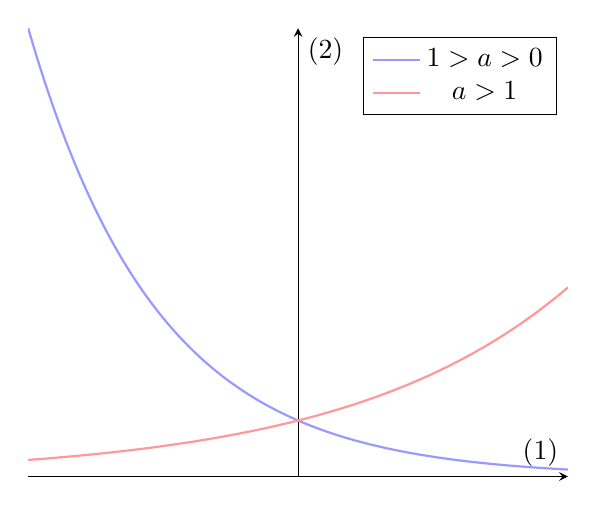
\begin{tikzpicture}
\begin{axis}[axis lines=middle, ticks = none,
ymin = 0,
xlabel = (1),
ylabel = (2)]
\addplot[color=blue!40,thick, domain=-3:3, samples=1000]{2*0.5^x};
\addplot[color=red!40,thick, domain=-3:3, samples=1000]{2*1.5^x};
\legend{$1>a>0$,$a>1$}
\end{axis}
\end{tikzpicture}
\caption{Eksponentiel vækst i de to tilfælde, at $1>a>0$ og $a>1$.}
\label{fig:eksp}
\end{figure}

\section*{Eksponentiel regression}
Har vi data, hvor vi forventer at kunne beskrive det ved en lineær sammenhæng, så kan vi "fitte" den bedste rette linje på det data. Dette kalder vi lineær regression. Vi kan gøre det præcist samme med eksponentiel data, altså data, vi forventer kan beskrives ved eksponentiel vækst. Vi udnytter logaritmen til at linearisere modellen. Betragt derfor en eksponentiel funktion $f(x) = b\cdot a^x$. Tager vi den naturlige logaritme af denne fås
\begin{align*}
\ln(f(x)) &= \ln\left(b\cdot a^x\right) \\
 &= \ln(b)+\ln(a^x)\\
 &= \underbrace{\ln(b)}_{=\beta}+x\underbrace{\ln(a)}_{=\alpha}.
\end{align*}
Vi har derfor en lineær sammenhæng mellem $F(x) = \ln(f(x))$ og $x$ givet ved
\begin{align*}
F(x) = \alpha x + \beta,
\end{align*}
hvor $\alpha = \ln(a)$ og $\beta = \ln(b)$. Vi kan derfor bruge nøjagtigt samme værktøj til eksponentiel regression som til lineær regression. Vi tager altså logaritmen af alt vores data. Vi laver så lineær regression, og til sidst tager vi $e$ og opløfter i vores regression. 

\begin{exa}
Vi antager, at det daglige antal smittede med omikron-varianten af Covid-19 vokser eksponentielt. På Fig. \ref{fig:Omik} ses blandt andet det daglige antal bekræftede smittede af omikron-varianten. Data er hentet tors. d. 16. dec. 2021. 

\begin{figure}[H]
\center
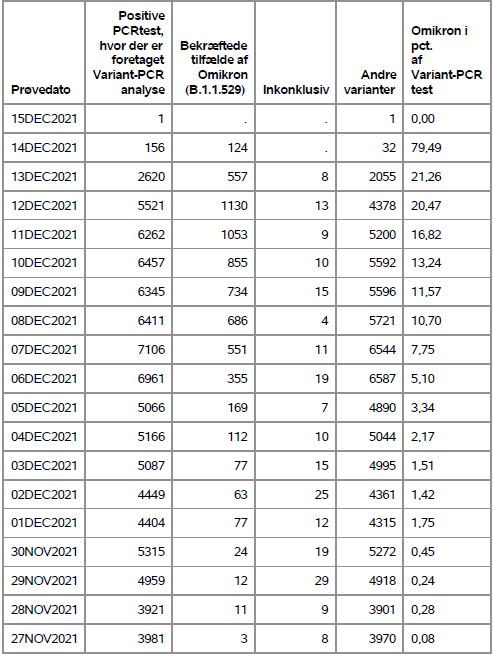
\includegraphics[scale=1]{Billeder/Omicron_ssi}
\caption{Omikron-data}
\label{fig:Omik}
\end{figure}

Uden at tage forbehold for variationen i testintensitet så vil vi fitte en eksponentiel regressionslinje på antallet af omikron-bekræftede som funktion af tiden. Dette kan ses på Fig. \ref{fig:Omikreg1}

\begin{figure}
\center
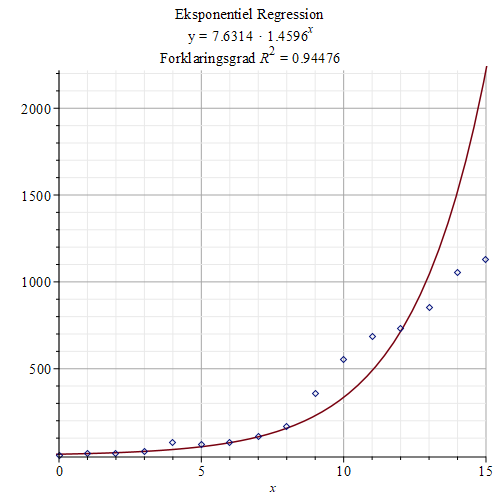
\includegraphics[scale=0.6]{Billeder/expreg}
\caption{Eksponentiel regression på Omikron-varianten}
\label{fig:Omikreg1}
\end{figure}

\end{exa}

\section*{Opgave 1}
Vi betragter igen Omikron-datasættet.
\begin{enumerate}[label=\roman*)]
\item Vi skal tage højde for den daglige variation i testintensitet. Derfor tager vi antallet af bekræftede smittede (Søjle 3) og dividerer det med det daglige antal Variant-PCR-tests (Søjle 2). Dette giver den procentvise andel af omicron/variant-pcr-test (Søjle 6). Lav nu exponentiel regression på dette. Ser det rigtigere ud?
\item Det ser ud til at smitten vokser meget tæt på eksponentielt i starten, men flader lidt ud senere. Har I et bud på, hvorfor dette sker? Der er ikke nødvendigvis noget rigtigt svar. 
\item I stedet for at bruge \texttt{ExpReg} i Maple, så skal i tage $\ln$ af al dataen og plotte det op mod tiden. Ser det lineært ud? Brug nu lineær regression på dette data. Du får så en funktion $F(x)=ax+b$. Bestem nu $f(x) = e^{ax+b}$ og sammenlign denne med regressionen fra eksemplet. Kommentér på resultatet.  
\item Er det realistisk at omikron-variantens vækst kan blive ved med at være eksponentiel? Hvilke eventuelle begrænsende faktorer er der?
\end{enumerate}
